\documentclass[11pt,a4paper,oneside]{scrartcl}
\usepackage[utf8]{inputenc}
\usepackage[english]{babel}
\usepackage{amsmath}
\usepackage{amsfonts}
\usepackage{amssymb}
\usepackage{graphicx}
\usepackage{lmodern}

\usepackage{pgfplots}
\pgfplotsset{compat=newest}
\usepackage{tikz}

\pgfplotsset{
    legend entry/.initial=,
    every axis plot post/.code={%
        \pgfkeysgetvalue{/pgfplots/legend entry}\tempValue
        \ifx\tempValue\empty
            \pgfkeysalso{/pgfplots/forget plot}%
        \else
            \expandafter\addlegendentry\expandafter{\tempValue}%
        \fi
    },
}


\usepackage[lmargin = 2cm,rmargin=2cm, tmargin = 2cm,bmargin=2cm]{geometry}

% Listings options
\usepackage{listings}
\usepackage{xcolor}
\definecolor{zebg}{rgb}{1,1,.8} %elfenbeinfarbig

\lstset{language=Matlab, numbers=left, numberstyle=\tiny, basicstyle=\footnotesize,showstringspaces=false,%
 numberblanklines=false, frame=single, backgroundcolor=\color{zebg},xleftmargin=0cm, linewidth=1.11\linewidth}



\author{Lars Schiller}
\title{Simulation of a wolf population by the
E-10-Simulation GmbH}

\begin{document}
\maketitle
\tableofcontents

\section{Introduction and task description}
In 2011, wolves where sighted in Luneburg Heath for the first time (after quite a long
period). The E-10-Simulation GmbH was asked by the Ministry of Food, Agriculture and
Consumerism of Lower Saxony to forecast the development of the wolf population over
the next 15 years.

The E-10-Simulation GmbH asks all interested students to submit a simulation proposal.
The main task consists of modelling the development of the population mathematically,
choosing a suitable solver for the simulation, writing a corresponding software program
and evaluating the results. Further technical details and specifications are listed in the
attachment.


\section{Mathematical model of the wolf population}

From the Task Sheet it is known, that the population size of the wolves in Luneburg Heath in the year 2011 is equal to 20. This yields to equation~\ref{eq:init}:
\begin{equation}
w(t_0) = w_0 = 20 \qquad,\quad t_0 = 2011.
\label{eq:init}
\end{equation}
Furthermore it is known, that the growth rate of a wolf population is proportional to the current population with respect to a constant factor. Due to a limited amount of food, the growth rate will be also proportional to $1-b*w$.  This yields to equation~\ref{eq:prop1} and equation~\ref{eq:prop2}:

\begin{equation}
\dot{w} \sim a\cdot w \qquad,\quad a = 0.055,
\label{eq:prop1}
\end{equation}

\begin{equation}
\dot{w} \sim 1-b\cdot w \qquad,\quad b = \frac{1}{250}.
\label{eq:prop2}
\end{equation}

In order to obtain a differential equation which describes the behaviour of the wolf population adequate, and therefore fulfils  equation~\ref{eq:prop1} and \ref{eq:prop2}, one can simply multiply the both restrictions, which corresponds with a logical \texttt{AND}-connector. This yields to the following ordinary differential equation (ODE):
\begin{equation}
\dot{w} = \left(aw\right)\left(1-bw\right).
\label{eq:ODE}
\end{equation}

In the following section this ODE will be solved by different numerical methods.


\section{Solutions of the mathematical model obtained by different numerical methods}

The following different numerical methods are used to solve the ODE:
\begin{enumerate}
    \item the Simple \textit{Euler}-Method,
    \item the advanced \textit{Euler}-Method and
    \item the \textit{Runge-Kutta}-Method.
\end{enumerate}

\subsection{Simple \textit{Euler}-Method}
This is the most simple method to solve an ODE with initial condition. It is based on the \textit{Taylor}-series expansion. The \textit{Taylor}-series expansion says, a function $f(x)$ can be described around a working point $x_0$ as the sum of its derivatives, with the following rule
\begin{eqnarray}
        Tf(x)\bigg|_{x_0} &=&    \sum\limits_{n=0}^{\infty}\frac{f^{(n)}(x_0)}{n!}(x-x_0)^n \\
        &=& f(x_0) + f^{(1)}(x_0)(x-x_0) + \frac{1}{2}f^{(2)}(x_0)(x-x_0)^2 + \cdots + \frac{1}{\infty!}f^{(\infty)}(x_0)(x-x_0)^\infty , \label{eq:taylor}
\end{eqnarray}
where $f^{(n)}$ denotes the $n$-th derivative of $f$ with respect to $x$.
For an initial value problem with the form 
$$y' = f(x,y) \quad , \quad y(x_0) = y_0$$
the linearised (only the first derivative is respected) and discretized version of equation~\ref{eq:taylor} is the following:
\begin{equation}
    y_{n+1} = y_n + \frac{\delta}{\delta x}y(x_n)\cdot \underbrace{ \big(x_{n+1}-x_n\big) }_{\textnormal{step size: } h_n} = y_n + f(x_n,y_n) \cdot  h_n.
    \label{eq:taylor_lin}
\end{equation}
Since the first derivative of $f$ is given and we also know the initial value, equation~\ref{eq:taylor_lin} can be used within a \texttt{while}-loop to calculate the values of the desired function. The only thing we don't know is the step size. The most simple way is to set the step size to a constant value:
$$h_n=h_0 .$$
The solution depends strongly on this step size $h_0$. In figure~\ref{fig:ODEsol} the blue curve represents the result of this method.

\subsection{Advanced \textit{Euler}-Method}
The main idea of this method is equal to the simple \textit{Euler}-Method. Based on the linearised \textit{Taylor} series expansion, the solution is calculated recursively. But this time we change the step size individually, with respect to the changes in the right hand side of the ode. Therefore the changes of step size will be proportional to the second derivative of the desired function. In every calculation step the next value of the solution is calculated with the current step size (like the simple \textit{Euler}-method) and stored in $y_{n+1}$. Furthermore the its calculated by doing two steps with half the current step size (like doing the simple \textit{Euler} twice) and stored in $\tilde{y}_{n+1}$. The difference of these two values is an good estimator for the local error we do. Therefore the local error estimator $\varphi$ is defined:
\begin{equation}
\varphi(x_n,y_n,h_n) = 2(\tilde{y}_{n+1}-y_{n+1})
\end{equation}
If the local error is great the step size decreases, and if its small the step size increases.

Another important feature of the advanced \textit{Euler}-method is the usage of a linear combination of the both calculated values ($y_{n+1}$ and $\tilde{y}_{n+1}$) as the next value of the solution $\hat{y}_{n+1}$. Therefore the order of the method is increased. The local error of the simple \textit{Euler}-method is a function of $h_n^2$. In comparison to that the advanced method holds a local error $\hat{\varepsilon}_n = \mathcal O (h_n^3)$.
 The mathematical explanation for this can be found in the lecture Script on page~15ff.
The principle scheme of the advanced \textit{Euler}-method is represent in figure~\ref{fig:adv_euler} and the solution of the given problem calculated with this method is represented by the red curve in figure~\ref{fig:ODEsol}.

\begin{figure}
\begin{center}

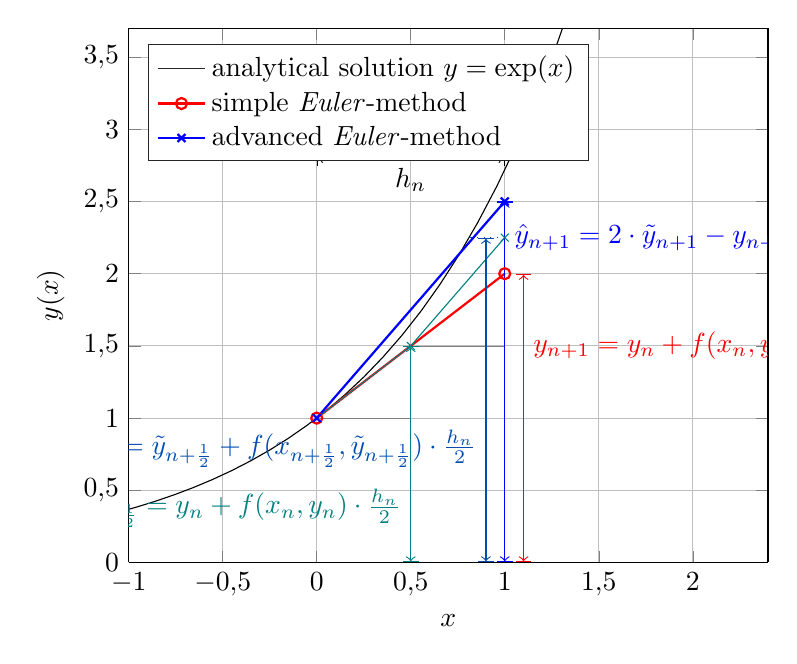
\begin{tikzpicture}[]

\begin{axis}[%
width = .8\textwidth,
separate axis lines,
ticklabel style={% gilt für x und y
    /pgf/number format/.cd,
    use comma,% Komma als Dezimaltrenner
    1000 sep = {}% keine Tausendertrennung 
  },
xmin=-1,
xmax=2.4,
xlabel={$x$},
xmajorgrids,
ymin=0,
ymax=3.7,
ylabel={$y(x)$},
ymajorgrids,
legend style={at={(.03,.97)},anchor=north west,draw=white!15!black,fill=white,legend cell align=left}
]
\addplot[samples = 100,legend entry = {analytical solution $y = \exp(x)$}]{exp(x)};

\addplot[thick,mark = o, color = red,legend entry = simple \textit {Euler}-method] coordinates {(0,1) (1,1+1*1)};
\draw[|<->|] (axis cs:0,2.8)--(axis cs: 1,2.8)node[midway,below]{$h_n$};

% Adv Euler
\addplot[mark = x, color = blue!50!green] coordinates {(0,1) (.5,1.5) (1,1.5+1.5*.5)};
\draw[red,|<->|] (axis cs: 1.1,0)--(axis cs: 1.1,2)node[near end,right]{$y_{n+1} = y_n + f(x_n,y_n)\cdot h_n$};


\draw[help lines] (axis cs:0,1)--(axis cs: .5,1)(axis cs: .5,1.5)--(axis cs: 1,1.5);
\draw[blue!50!green,|<->|] (axis cs: 0.5,0)--(axis cs: .5,1.5)node[near start,left]{$\tilde{y}_{n+\frac{1}{2}} = y_n + f(x_n,y_n)\cdot \frac{h_n}{2}$};
\draw[blue!70!green,|<->|](axis cs: .9,0)--(axis cs: .9,2.25)node[pos=.35,left]{$\tilde{y}_{n+1} = \tilde{y}_{n+\frac{1}{2}} + f(x_{n+\frac{1}{2}},\tilde{y}_{n+\frac{1}{2}})\cdot \frac{h_n}{2}$};
%help lines
\draw[blue!70!green,dotted] (axis cs: 1,2.25)--(axis cs: .8,2.25);

\addplot[thick,mark = x, color = blue,legend entry = advanced \textit{Euler}-method] coordinates {(0,1) (1,2*2.25-2)};
\draw[blue,|<->|](axis cs: 1,0)--(axis cs: 1,2.5)node[pos=.9,right]{$\hat{y}_{n+1} = 2\cdot \tilde{y}_{n+1} - y_{n+1}$};

\end{axis}
\end{tikzpicture}
\end{center}
\caption{principle scheme of the advanced \textit{Euler}-Method by means of the initial value problem: $\dot{y}=y, y(0)=1$}
\label{fig:adv_euler}
\end{figure}


\subsection{\textit{Runge-Kutta}-Method}

This solver is implemented by the Mathwork guys. I hope to understand the mathematics of \texttt{ode45} within this lecture.
The result of this solver is represented by the green curve in figure~\ref{fig:ODEsol} and will be used as an reference for the exact solution in the evaluation.



\begin{figure}
% This file was created by matlab2tikz v0.4.7 running on MATLAB 8.4.
% Copyright (c) 2008--2014, Nico Schlömer <nico.schloemer@gmail.com>
% All rights reserved.
% Minimal pgfplots version: 1.3
% 
% The latest updates can be retrieved from
%   http://www.mathworks.com/matlabcentral/fileexchange/22022-matlab2tikz
% where you can also make suggestions and rate matlab2tikz.
% 
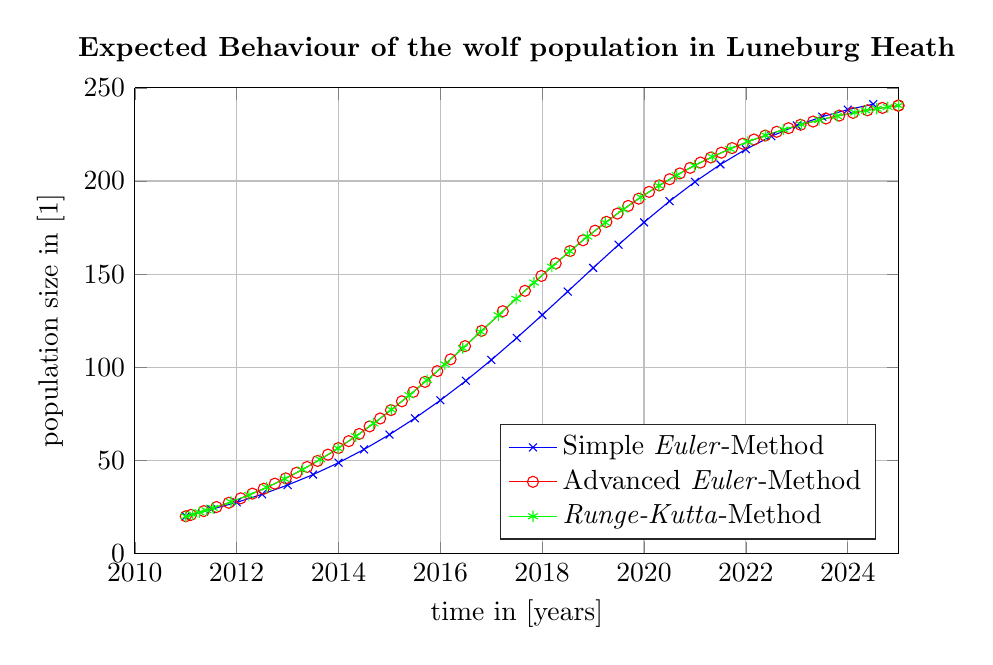
\begin{tikzpicture}

\begin{axis}[%
width=0.8\textwidth,
height=0.487748079877112\textwidth,
scale only axis,
separate axis lines,
ticklabel style={% gilt für x und y
    /pgf/number format/.cd,
    use comma,% Komma als Dezimaltrenner
    1000 sep = {}% keine Tausendertrennung 
  },
xmin=2010,
xmax=2025,
xlabel={time in [years]},
xmajorgrids,
ymin=0,
ymax=250,
ylabel={population size in [1]},
ymajorgrids,
title style={font=\bfseries},
title={Expected Behaviour of the wolf population in Luneburg Heath},
legend style={at={(0.97,0.03)},anchor=south east,draw=white!15!black,fill=white,legend cell align=left}
]
\addplot [color=blue,solid,mark=x,mark options={solid},legend entry=Simple \textit{Euler}-Method]
  table[row sep=crcr]{%
2011	20\\
2011.5	23.7306\\
2012	27.4612\\
2012.5	31.815871493772\\
2013	36.7720404968602\\
2013.5	42.4017739526279\\
2014	48.7606847809388\\
2014.5	55.8995390875927\\
2015	63.8575307744998\\
2015.5	72.6569832051727\\
2016	82.2970145538068\\
2016.5	92.746918722581\\
2017	103.939898755141\\
2017.5	115.76812187986\\
2018	128.080295781796\\
2018.5	140.683051219586\\
2019	153.34723127146\\
2019.5	165.819634255964\\
2020	177.839817618629\\
2020.5	189.160369918048\\
2021	199.567895347687\\
2021.5	208.901245809522\\
2022	217.063659915072\\
2022.5	224.026566066828\\
2023	229.824634193015\\
2023.5	234.543631694768\\
2024	238.304073304538\\
2024.5	241.244104628941\\
};

\addplot [color=red,solid,mark=o,mark options={solid},legend entry = Advanced \textit{Euler}-Method]
  table[row sep=crcr]{%
2011	20\\
2011.1	20.7588045957355\\
2011.35269939034	22.7922714072617\\
2011.60241324646	24.9761690047069\\
2011.84421607724	27.2664449711803\\
2012.07888868719	29.6636120892728\\
2012.30731733974	32.1702611253808\\
2012.53030997845	34.7894041945468\\
2012.74860787192	37.5244677609932\\
2012.96290126063	40.3793590279926\\
2013.17384339077	43.3585512439324\\
2013.3820635046	46.4671911996922\\
2013.58817949573	49.7112361543698\\
2013.79281096604	53.0976305405774\\
2013.99659353494	56.6345374385869\\
2014.20019549024	60.3316470213305\\
2014.40433829832	64.2005957151737\\
2014.60982323594	68.2555489015536\\
2014.81756771431	72.514032720103\\
2015.02865723311	76.9981591854389\\
2015.24442338887	81.7364994276001\\
2015.4665673747	86.7670816087546\\
2015.69736791096	92.1424693160347\\
2015.9400588988	97.9390145243256\\
2016.19958666252	104.275436352186\\
2016.48435287705	111.355592157385\\
2016.81116770996	119.589935461715\\
2017.22582127016	130.098793212881\\
2017.6610064742	141.048643314034\\
2017.9842620129	149.029796760596\\
2018.26445365066	155.788480191419\\
2018.54639496142	162.400779591682\\
2018.80058261894	168.172135982985\\
2019.03655236487	173.349439939491\\
2019.26080537419	178.095430546656\\
2019.47703595835	182.501377560677\\
2019.68761454303	186.62474908879\\
2019.89421705673	190.505051557178\\
2020.09811172343	194.171063720855\\
2020.30030957651	197.644632953654\\
2020.50165188244	200.942870611851\\
2020.70286486079	204.079512265206\\
2020.90459606801	207.06580570254\\
2021.10743990505	209.911115127969\\
2021.31195641246	212.623346357328\\
2021.51868582126	215.209254592167\\
2021.72816040442	217.674672602811\\
2021.94091464921	220.02468344916\\
2022.15749446478	222.263753627067\\
2022.37846595998	224.395837395233\\
2022.60442422548	226.424459742261\\
2022.83600250487	228.352783281947\\
2023.07388212866	230.183662900922\\
2023.31880360602	231.919690976366\\
2023.57157932045	233.563235278247\\
2023.83310836184	235.116471172811\\
2024.10439415345	236.581409388956\\
2024.3865657136	237.959920355632\\
2024.68090364526	239.25375593955\\
2024.98887230365	240.464569290724\\
2025	240.505868469475\\
};


\addplot [color=green,solid,mark=asterisk,mark options={solid},
			legend entry = \textit{Runge-Kutta}-Method
			]
  table[row sep=crcr]{%
2011	20\\
2011.13466393779	21.0280781484263\\
2011.26932787557	22.1039254447645\\
2011.40399181336	23.2292301255014\\
2011.53865575114	24.4056874165653\\
2011.88865575114	27.7146733938813\\
2012.23865575114	31.4100679954852\\
2012.58865575114	35.5194175064827\\
2012.93865575114	40.0675883191595\\
2013.28865575114	45.0757553311377\\
2013.63865575114	50.5594469358106\\
2013.98865575114	56.5262203434971\\
2014.33865575114	62.9745267564955\\
2014.68865575114	69.8928375329184\\
2015.03865575114	77.2572216534417\\
2015.38865575114	85.0311826384367\\
2015.73865575114	93.1655378619178\\
2016.08865575114	101.599054440274\\
2016.43865575114	110.258806702804\\
2016.78865575114	119.064403533459\\
2017.13865575114	127.929914216619\\
2017.48865575114	136.766050395547\\
2017.83865575114	145.484695641044\\
2018.18865575114	154.003227647099\\
2018.53865575114	162.246631064978\\
2018.88865575114	170.149014275696\\
2019.23865575114	177.65709074745\\
2019.58865575114	184.730019160995\\
2019.93865575114	191.339706438054\\
2020.28865575114	197.470428977333\\
2020.63865575114	203.117640481044\\
2020.98865575114	208.28582980074\\
2021.33865575114	212.987825513077\\
2021.68865575114	217.243543358233\\
2022.03865575114	221.076550351457\\
2022.38865575114	224.513320322601\\
2022.73865575114	227.582878497175\\
2023.08865575114	230.315679885932\\
2023.43865575114	232.740654744096\\
2023.78865575114	234.886101230737\\
2024.13865575114	236.779846198391\\
2024.35399181336	237.831462851536\\
2024.56932787557	238.803381396511\\
2024.78466393779	239.70100694581\\
2025	240.529518488111\\
};
%\addlegendentry{Runge-Kutta-Method}

\end{axis}
\end{tikzpicture}%
\caption{Solutions of the ODE (step size of simple \textit{Euler}-method: $h_0=.5$)}
\label{fig:ODEsol}
\end{figure}




\section{Description and evaluation of the results}

The results of all solvers are reasonable. First the wolf population grows slowly and than faster and faster, which corresponds perfectly with the constraint given in equation~\ref{eq:prop1}. When the upper limit of the population (250) is almost reached, the slope begins to decrease, which is demand by the constraint given in equation~\ref{eq:prop2}. 

\begin{table}[h]
\centering
\begin{tabular}{c|ccc}
criteria & Simple \textit{Euler} ($h_0=.5$) & Advanced \textit{Euler} & \texttt{ode45} \\
\hline
supporting points & 29 & 21 & 45 \\
calculation time [sec] & 0.0057 & 0.0061 & 0.1710 \\
global error & -2.97  & 0.20 & (reference) 

\end{tabular}

\caption{Evaluation of the results}
\label{tab:eva}
\end{table}

In table~\ref{tab:eva} some evaluation criteria are listed. The calculation time of the simple \textit{Euler}-method and the advanced one are nearly the same. In figure~\ref{fig:ODEsol} one can see that the solution of advanced \textit{Euler} almost perfectly fits the one of \texttt{ode45}, which can be treated as exact solution. The solution of the simple method is not that exact. Its too inert to realize the changes. Furthermore the advanced method needs less supporting points than the simple method. Therefore the storage space which is needed will be much smaller. 

In summary one can say the advanced \textit{Euler}-method gives much more qualitative results, needs less storage space and the computational effort is at least for this case not really greater than the one of the simple method.



\end{document} 